\chapter{Implementierung}
\label{chap:implementierung}

In diesem Kapitel werden die Details der Software- und Hardware-Implementierung 
des LED-Röhrensystems beschrieben. Es werden die Entwicklungsumgebung, 
die Projektstruktur, die Datenmodelle, die gemeinsamen Softwarekomponenten 
sowie die spezifischen Implementierungen für Bridge- und Tube-Firmware erläutert. 
Abschließend wird das Hardware-Design mit Fokus auf die Leiterplatten 
und den mechanischen Aufbau vorgestellt.

\section{Entwicklungsumgebung und Projektstruktur}
\label{sec:entwicklungsumgebung}

Die Firmware wurde mit PlatformIO als Build- und
Projektverwaltungssystem unter Verwendung des Arduino-Frameworks für
ESP32 entwickelt. Die Projektkonfiguration definiert zwei
Zielumgebungen, die unterschiedliche Hardwareplattformen adressieren:
\texttt{led\_tube} für ein Seeed XIAO ESP32-S3 sowie \texttt{bridge}
für ein ESP32 DevKitC. Beide Umgebungen teilen sich eine gemeinsame
Basiskonfiguration (Plattform, Framework, Monitorrate und
Bibliotheksabhängigkeiten), wodurch ein konsistenter Build-Prozess für
beide Gerätetypen sichergestellt wird.

Die Trennung zwischen Röhren- und Bridge-Firmware erfolgt über
bedingte Kompilierung mittels Präprozessormakro \texttt{DEVICE\_MODE}.
Der jeweilige Wert wird build-seitig gesetzt
(\texttt{-D DEVICE\_MODE=0} für Tube, \texttt{-D DEVICE\_MODE=1} für
Bridge) und in der Quellbasis über symbolische Konstanten ausgewertet.
Dadurch werden hardwarespezifische Pinbelegungen, Treiber und
Laufzeitpfade bereits zur Compile-Zeit selektiert. Dieses Vorgehen
reduziert Laufzeitverzweigungen und vermeidet die Einbindung nicht
benötigter Komponenten in das jeweilige Ziel-Binary.

Die zentrale Ablaufsteuerung ist in einer gemeinsamen
\texttt{setup()}/\texttt{loop()}-Struktur organisiert. Gemeinsame
Funktionen wie Menübedienung und ESP-NOW-Kanalsynchronisierung werden
in beiden Gerätevarianten ausgeführt, bridge-spezifische Funktionen
(DMX-Eingang und Generierung der Tube-Payload) werden ausschließlich
im Bridge-Build kompiliert. Innerhalb der Hauptschleife wählt eine
\texttt{switch}-Verzweigung anhand des im Menü gesetzten Betriebsmodus
den jeweils aktiven Datenpfad aus.

Die externen Bibliotheken umfassen insbesondere \texttt{FastLED}
(LED-Ansteuerung), \texttt{esp\_dmx} (DMX512-Empfang), \texttt{Ethernet}
und \texttt{ArtNet} (Art-Net-Empfang über das W5500-Modul) sowie
\texttt{Adafruit GFX}/\texttt{Adafruit SSD1306} (OLED-Ausgabe). Die
Abhängigkeiten sind in der Projektkonfiguration explizit versioniert,
um reproduzierbare Builds zu gewährleisten.

\section{Datenmodell und Paketformate}
\label{sec:datenmodell}

Der Datenaustausch zwischen den Softwarekomponenten basiert auf zwei
klar abgegrenzten DTO-Strukturen (\textit{Data Transfer Objects}).
Diese Trennung ermöglicht eine einheitliche Schnittstelle zwischen dem
DMX-Eingang, der internen Effektlogik und der Ausgabe an die
LED-Controller. Die Formatwahl folgt dem Ziel, einerseits die
Funkübertragung kompakt zu halten und andererseits ausreichend Struktur
für unterschiedliche Betriebsarten bereitzustellen.

\subsection{TubeInput}
\label{subsec:tubeinput}

\texttt{TubeInput} beschreibt den Steuerzustand einer einzelnen Röhre
und umfasst vier Byte: Effektkennung sowie RGB-Werte. Das Format ist auf effektbasierte Ansteuerung
ausgelegt und dient als kleinstes semantisches Steuerobjekt im System.
Durch die feste Feldreihenfolge kann die Struktur ohne zusätzliche
Serialisierung direkt aus empfangenen Bytefolgen rekonstruiert werden.

\subsection{DmxFrame}
\label{subsec:dmxframe}

\texttt{DmxFrame} bildet den Transportrahmen für
drahtlose Übertragung. Die Struktur enthält ein Größenfeld
(\texttt{size}), ein Adressfeld (\texttt{start\_address}) sowie ein
Nutzdatenarray mit bis zu 240 Byte. Die Obergrenze der Nutzdaten
orientiert sich an der Paketgröße von ESP-NOW, die in der ersten
Generation des Protokolls 250 Byte beträgt
(Abschnitt~\ref{subsec:espnow-protokoll}). Die verbleibenden zehn Byte
stehen für den Rahmen und dessen beide Kopfbyte zur Verfügung. Beide
Kopffelder werden ausgewertet: \texttt{size} begrenzt die übertragenen
und verarbeiteten Daten, \texttt{start\_address} bildet die Grundlage
der im folgenden Abschnitt beschriebenen Offsetberechnung.

Im Master-Betrieb der Bridge wird die Nutzlast deterministisch
aufgebaut: Für jede der \(n\) angesteuerten Röhren werden vier
aufeinanderfolgende Byte abgelegt, bestehend aus Effektkennung sowie
den RGB-Werten (\texttt{Effekt}, \texttt{R}, \texttt{G}, \texttt{B}).
Ein zusätzlicher globaler Header wird in dieser Betriebsart nicht
vorangestellt, sodass sich eine Payload-Länge von 4n
Byte ergibt. Das Größenfeld wird entsprechend auf \(4n\) gesetzt und das
Adressfeld auf den Startwert~\texttt{1}. Die feste Datensatzlänge von
vier Byte pro Röhre vereinfacht die Indexberechnung und ermöglicht eine
konstante Zugriffskomplexität. Abbildung~\ref{fig:dmxframe-layout} zeigt
den resultierenden Aufbau eines Frames.

\begin{figure}[H]
    \centering
    \begin{tikzpicture}[x=1cm, y=1cm,
        byte/.style    = {draw, minimum height=0.9cm, minimum width=1.25cm,
                          align=center, font=\footnotesize, inner sep=1pt},
        kopf/.style    = {byte, fill=black!12, minimum width=2.0cm},
        nutz/.style    = {byte, fill=black!3},
        klammer/.style = {decorate, decoration={brace, amplitude=4pt, mirror}},
        klammero/.style= {decorate, decoration={brace, amplitude=4pt}},
        note/.style    = {font=\footnotesize, align=center}]

        \node[kopf] (size) at (0,0) {\texttt{size}};
        \node[kopf, right=0pt of size] (addr) {\texttt{start\_}\\\texttt{address}};

        \node[nutz, right=0pt of addr] (e1) {Effekt};
        \node[nutz, right=0pt of e1]   (r1) {R};
        \node[nutz, right=0pt of r1]   (g1) {G};
        \node[nutz, right=0pt of g1]   (b1) {B};

        \node[byte, draw=none, minimum width=0.9cm, right=0pt of b1] (luecke) {$\cdots$};

        \node[nutz, right=0pt of luecke] (en) {Effekt};
        \node[nutz, right=0pt of en]     (rn) {R};
        \node[nutz, right=0pt of rn]     (gn) {G};
        \node[nutz, right=0pt of gn]     (bn) {B};

        \draw[klammero] (e1.north west) -- (bn.north east)
            node[note, midway, above=6pt] {Nutzdaten: $4n$ Byte, höchstens 240\,Byte};

        \draw[klammer] (size.south west) -- (addr.south east)
            node[note, midway, below=6pt] {Kopf\\2\,Byte};
        \draw[klammer] (e1.south west) -- (b1.south east)
            node[note, midway, below=6pt] {Röhre~1\\Adresse~1};
        \draw[klammer] (en.south west) -- (bn.south east)
            node[note, midway, below=6pt] {Röhre~$n$\\Adresse~$4n-3$};
    \end{tikzpicture}
    \caption{Aufbau eines \texttt{DmxFrame} im Master-Betrieb. Auf die beiden Kopfbyte
        folgt je Röhre ein Block fester Länge. Aus dieser Regelmäßigkeit ergibt sich die
        im folgenden Abschnitt beschriebene Offsetberechnung ohne dynamisches Parsen.}
    \label{fig:dmxframe-layout}
\end{figure}

\subsection{Adressierungsschema}
\label{subsec:adressierung}

Die Datenadressierung erfolgt paketintern über einen byteweisen
Offsetzugriff in Anlehnung an die DMX-Kanaladressierung. Jeder
\texttt{DmxFrame} führt mit \texttt{start\_address} die DMX-Adresse des
ersten Nutzdatenbytes mit. Eine empfangende Röhre berechnet aus ihrer
konfigurierten Adresse den relativen Offset als Differenz von
Geräteadresse und Frame-Startadresse und liest ab dieser Position vier
Byte als \texttt{TubeInput} aus. Vor dem Zugriff wird geprüft, dass der
Offset innerhalb der übertragenen Nutzdatenlänge liegt. Andernfalls wird
der Lesevorgang verworfen. Da die Master-Nutzlast je Röhre einen Block
von vier Byte belegt, werden Geräteadressen praktisch in Schritten von
vier vergeben. Dieses Schema erlaubt einen einfachen, indexbasierten
Zugriff ohne dynamische Parsing-Logik.


\section{Gemeinsame Softwarekomponenten}
\label{sec:gemeinsame-komponenten}

\subsection{Menü- und Bediensystem}
\label{subsec:menu}

Das Menü- und Bediensystem ist als geräteübergreifende Komponente
implementiert und kapselt die Erfassung der Benutzereingaben, die
Darstellung auf dem OLED-Display sowie die persistente Speicherung der
Konfiguration. Die Bedienung erfolgt über drei Taster (UP, DOWN,
ENTER), deren Betätigung über Hardware-Interrupts erfasst wird. 
Die fallende Flanke der mit internem Pull-Up beschalteten Eingänge 
löst die jeweilige ISR (\textit{Interrupt Service Routines}) aus, wodurch die
Eingabeverarbeitung nicht-blockierend in den Programmablauf integriert
ist. Um mechanisches Prellen zu unterdrücken, verwirft eine
Entprellroutine Auslösungen, die innerhalb einer Sperrzeit von 200~ms
nach der letzten gültigen Betätigung auftreten.

Für die fortlaufende Werteänderung bei gehaltener Taste ist eine
Autoincrement-Funktion realisiert: Wird ein Taster länger als 1000~ms
gehalten, wiederholt die Hauptschleife die zugehörige Aktion in
Intervallen von 50~ms. Da die ISRs ausschließlich die fallende Flanke
erfassen, wird das Loslassen der Taster durch zyklisches Abfragen der
Pin-Zustände in der Hauptschleife erkannt.

Die Menüeinträge sind über eine Klassenhierarchie mit gemeinsamer
Basisklasse \texttt{MenuItem} typisiert. Numerische Parameter
(\texttt{NumericMenuItem}) werden über ein Wertintervall mit
Überlaufverhalten definiert, Auswahlparameter
(\texttt{CategoryMenuItem}) bilden benannte Optionen auf interne Werte
ab, Knotenelemente (\texttt{MenuNode}) ermöglichen den Aufbau
hierarchischer Untermenüs und \texttt{BackMenuItem} dient als Rücksprung
aus einem Untermenü. Da \texttt{MenuNode} selbst wieder Zeiger auf
\texttt{MenuItem}-Objekte hält, lassen sich Untermenüs beliebig
schachteln, ohne dass die Navigationslogik die konkreten Eintragstypen
kennen muss (Abbildung~\ref{fig:menu-klassen}). Die Navigation zwischen
den Menüebenen wird über einen Stapelspeicher mit begrenzter Tiefe
verwaltet. Das Bediensystem unterscheidet einen Navigations- und einen
Bearbeitungsmodus, zwischen denen die ENTER-Taste umschaltet.

\begin{figure}[H]
    \centering
    \begin{tikzpicture}[x=1cm, y=1cm,
        klasse/.style = {archbox, text width=3.0cm, fill=black!3, minimum height=1.7cm},
        basis/.style  = {archbox, text width=4.6cm, fill=black!12, thick},
        erbt/.style   = {-{Triangle[open, length=3mm, width=3mm]}, thick},
        haelt/.style  = {{Diamond[open, length=2.6mm, width=2.0mm]}-{Latex[length=2mm]},
                         thick, dashed}]

        \node[basis] (menu) at (0.1,2.2)
            {\textbf{\texttt{Menu}}\\[2pt]\footnotesize \texttt{build\_menu\_tree()},
             Navigationsstapel, NVS-Zugriff};
        \node[basis] (item) at (0.1,0)
            {\textbf{\texttt{MenuItem}}\\[2pt]\footnotesize \texttt{increment()},
             \texttt{decrement()}, \texttt{get\_display\_value()}, \texttt{is\_node()}};

        \node[klasse] (num)  at (-5.0,-2.7) {\texttt{Numeric-}\\\texttt{MenuItem}\\[2pt]\footnotesize Wertintervall mit Überlauf};
        \node[klasse] (cat)  at (-1.6,-2.7) {\texttt{Category-}\\\texttt{MenuItem}\\[2pt]\footnotesize benannte Optionen};
        \node[klasse] (back) at ( 1.8,-2.7) {\texttt{BackMenuItem}\\[2pt]\footnotesize Rücksprung};
        \node[klasse] (nod)  at ( 5.2,-2.7) {\texttt{MenuNode}\\[2pt]\footnotesize Untermenü mit Kindliste};

        % Vererbungsbaum mit gemeinsamem Stamm
        \coordinate (stamm) at (0.1,-1.5);
        \draw[thick] (-5.0,-1.5) -- (5.2,-1.5);
        \foreach \k in {num,cat,back,nod} \draw[thick] (\k.north) -- (\k.north |- stamm);
        \draw[erbt] (stamm) -- (item.south);

        % MenuNode hält selbst wieder MenuItem-Zeiger (Kompositum)
        \draw[haelt] (nod.east) -- (7.4,-2.7) -- (7.4,0) -- (item.east);
        \node[beschr, anchor=west] at (7.5,-1.6) {\texttt{MenuItem**}};

        \draw[link] (menu.south) -- (item.north)
            node[beschr, midway, right=1mm] {baut und durchläuft den Baum};
    \end{tikzpicture}
    \caption{Klassenstruktur des Bediensystems. Alle Eintragstypen leiten von
        \texttt{MenuItem} ab \texttt{MenuNode} hält seinerseits eine Liste solcher
        Einträge, wodurch die Menüstruktur rekursiv aufgebaut ist und
        \texttt{Menu} sie unabhängig vom konkreten Typ verwalten kann.}
    \label{fig:menu-klassen}
\end{figure}

Die verfügbaren Einträge werden modusabhängig zur Laufzeit aufgebaut:
Bei jedem Wechsel des Betriebsmodus erzeugt die Methode
\texttt{build\_menu\_tree()} die für den aktiven Modus relevante Auswahl
an Einträgen neu. Dadurch werden dem Bediener ausschließlich die im
jeweiligen Modus wirksamen Parameter angezeigt.

Die Anzeige erfolgt auf einem monochromen SSD1306-OLED-Display, das über
I2C mit einer Taktrate von 400~kHz angebunden ist. Um die Buslast gering
zu halten und die Auslastung des Mikrocontrollers zu minimieren, 
wird das Display flag-gesteuert neu gezeichnet, d.\,h. eine
Neuzeichnung erfolgt nur nach einer tatsächlichen Zustandsänderung. Im
Bearbeitungsmodus wird der aktive Eintrag zur visuellen Abgrenzung
invertiert dargestellt.

Sämtliche Konfigurationswerte werden im nichtflüchtigen Speicher (NVS)
des ESP32 abgelegt, wofür die \texttt{Preferences}-Bibliothek unter einem
gemeinsamen Namensraum genutzt wird. Beim Systemstart werden die
gespeicherten Werte geladen, sodass die zuletzt gewählte Konfiguration
ohne erneute Eingabe verfügbar ist. Um Schreibzugriffe aus dem
Interrupt-Kontext herauszuhalten, wird eine Wertänderung in der ISR
lediglich vorgemerkt. Der eigentliche Schreibvorgang in den
Flash-Speicher wird anschließend in der Hauptschleife ausgeführt.

\subsection{LED-Steuerung und Effekte}
\label{subsec:led-steuerung}

Die LED-Steuerung kapselt die \texttt{FastLED}-Bibliothek, welche die
zeitkritische Ansteuerung der adressierbaren LEDs übernimmt. Die
LED-Kette wird zur Initialisierung mit \texttt{NUM\_LEDS} Pixeln und
festgelegter Farbreihenfolge an einem dedizierten Daten-Pin registriert.
Die Übergabe der Eingangsdaten erfolgt über mehrfach überladene
\texttt{set\_input()}-Methoden, die einen Effektdatensatz 
(\texttt{TubeInput}) für den drahtlosen Empfang entgegennehmen 
und in den internen Zustand überführen.

Die zyklisch aufgerufene Methode \texttt{handle()} wählt anhand der gespeicherten Effektkennung den
auszuführenden Effekt aus und schreibt das Ergebnis abschließend über
\texttt{FastLED.show()} an die Hardware. Die implementierten
Effekte umfassen statische Farbdarstellung und Helligkeitsverläufe,
helligkeitsmodulierte Pulseffekte, positions- bzw. laufzeitbasierte
Lauflichter, Lauflichter mit exponentiell abklingendem Nachleuchten,
simulationsbasierte Effekte wie Feuer, Perlin-Rauschen und einen
springenden Ball sowie Strobo-, Blitz-, Funkel- und Regenbogeneffekte.
Helligkeitsverläufe werden über eine exponentielle Kennlinie (vierte
Potenz der normierten Helligkeit) berechnet, um weiche, visuell
gleichmäßige Helligkeitsübergänge zu erzeugen.

Die Effekte sind als reine Funktionen der verstrichenen Zeit
formuliert und nicht als Funktionen der Aufrufhäufigkeit. Die
Ablaufgeschwindigkeit ist dadurch unabhängig von der Schleifenrate,
die je nach Displayaktualisierung, Funkverkehr und Betriebsmodus
schwankt.

\subsection{Drahtlose Kommunikation (ESP-NOW)}
\label{subsec:espnow}

Die drahtlose Kommunikation ist im \texttt{WirelessDmxController}
gekapselt, der das ESP-NOW-Protokoll von Espressif verwendet. Zur
Initialisierung wird die WLAN-Schnittstelle in den Station-Modus
versetzt, die bestehende Access-Point-Funktion deaktiviert und ESP-NOW
initialisiert. Anschließend wird ein Empfangs-Callback registriert.
Adressiert wird ausschließlich über die Broadcast-MAC-Adresse
\texttt{FF:FF:FF:FF:FF:FF}, sodass alle Röhren in Reichweite gleichzeitig
erreicht werden.

Um die für den ESP32 maximal mögliche Sendeleistung von 20~dBm auszuschöpfen, 
muss keine Sendeleistungskonfiguration vorgenommen werden, da der ESP32 diese 
Leistung standardmäßig verwendet und nur bei gewünschter Drosselung explizit 
konfiguriert werden kann \cite{espressif_esp32_tx}.

Der im Menü wählbare logische Kanal (1 bis 3) wird über eine feste
Zuordnung auf die WLAN-Kanäle 1, 5 und 10 abgebildet. Diese Spreizung
verringert die gegenseitige Beeinflussung mehrerer parallel betriebener
Systeme. Ein Kanalwechsel wird zur Laufzeit über
\texttt{sync\_channel()} in der Hauptschleife erkannt und nur bei einer
tatsächlichen Änderung angewendet.

Der Empfang erfolgt im Interrupt-Kontext des Funktreibers: Der
registrierte Callback kopiert das eingegangene Paket unmittelbar in einen
internen \texttt{DmxFrame}-Puffer (Overwrite-Strategie), nachdem die
Rahmenlänge sowie die Konsistenz von Header und Nutzdatenlänge geprüft
wurden. Da der Callback statisch ist, wird der Zugriff auf die
Instanzdaten über ein Singleton-Muster hergestellt. Auf der Sendeseite
überträgt \texttt{write()} den Frame als Broadcast, wobei neben den
Nutzdaten die beiden Headerbyte (Größe und Startadresse) mitgesendet
werden.

\subsection{Nebenläufigkeit und Kernverteilung}
\label{subsec:nebenlaeufigkeit}

Ein wesentliches Entwurfsziel der Datenpfade ist die Entkopplung der
zeitkritischen Signalein- und -ausgabe von der zyklischen
Effektberechnung in der Hauptschleife. Hierzu werden zwei Mechanismen
genutzt: die interruptgesteuerte, asynchrone Verarbeitung der
Schnittstellen sowie die Verteilung der Arbeitslast auf die beiden Kerne
des ESP32. Abbildung~\ref{fig:datenpfad} zeigt den daraus folgenden
Datenpfad vom DMX-Eingang der Bridge bis zur Lichtausgabe der Röhre.

Der ESP32 ist ein Dual-Core-Mikrocontroller. Unter dem
Arduino-/FreeRTOS-Laufzeitsystem wird die Hauptschleife als
eigenständiger Task ausgeführt, der standardmäßig dem Applikationskern
zugeordnet ist, während der WLAN-Protokollstack, über den die
ESP-NOW-Übertragung abgewickelt wird, vom Laufzeitsystem auf dem
zweiten Kern (Protokollkern) betrieben wird. Das Senden und Empfangen
der Funkpakete erfolgt dadurch nebenläufig zur Effektberechnung und
blockiert die Hauptschleife nicht. Auf der Bridge kann somit der
Protokollkern bereits ein Funkpaket aussenden, während der
Applikationskern den nächsten DMX-Ausschnitt aufbereitet. Auf der Röhre
nimmt der Funkstack ein eingehendes Paket entgegen, ohne den laufenden
Render-Zyklus zu unterbrechen.

Der Empfang der ESP-NOW-Pakete wird über den registrierten Callback
realisiert, der asynchron aus dem Kontext des Funktreibers aufgerufen
wird. Da Funkempfang und Hauptschleife auf diese
Weise entkoppelt sind, dient der bereits beschriebene Overwrite-Puffer
als Übergabepunkt zwischen beiden Ausführungssträngen: Der Callback
aktualisiert den Puffer, sobald ein Paket eintrifft, und die
Hauptschleife liest stets den zuletzt gültigen Zustand.

Der DMX512-Empfang folgt demselben Prinzip der Entkopplung, ist jedoch
interruptgesteuert umgesetzt: Die \texttt{esp\_dmx}-Bibliothek erfasst
ein vollständiges Universum im Hintergrund über die UART-Hardware und
deren Interrupt-Routine. Die zeitkritische Erfassung des Bussignals ist
damit von der Ausführungszeit der Hauptschleife unabhängig. Diese pollt
den Treiber lediglich und entnimmt das fertig gepufferte Universum. Nach
demselben Muster werden die Benutzereingaben über Taster-Interrupts
erfasst und Flash-Schreibzugriffe aus dem Interrupt-Kontext heraus in die
Hauptschleife verlagert (vgl. Abschnitt~\ref{subsec:menu}), sodass die
Hauptschleife durchgängig kurze und gleichmäßige Zykluszeiten beibehält.

\begin{figure}[H]
    \centering
    \begin{tikzpicture}[x=1cm, y=1cm,
        stufe/.style  = {archbox, text width=2.6cm},
        async/.style  = {stufe, fill=black!12, thick},
        sync/.style   = {stufe, fill=black!3},
        puffer/.style = {stufe, draw, dashed, thick, fill=white}]

        % --- Bridge ---
        \node[async]  (b1) at (0,0)      {UART-ISR\\[1pt]\footnotesize \texttt{esp\_dmx}};
        \node[puffer] (b2) at (3.6,-1.35){Universumspuffer\\[1pt]\footnotesize im Treiber};
        \node[sync]   (b3) at (7.2,-2.7) {Hauptschleife\\[1pt]\footnotesize Ausschnitt wählen, \texttt{DmxFrame} füllen};
        \node[async]  (b4) at (10.8,0)   {ESP-NOW-Stack\\[1pt]\footnotesize Protokollkern};

        \draw[link] (b1) -- (b2);
        \draw[link] (b2) -- (b3) node[beschr, midway, below left=-1mm] {pollen};
        \draw[link] (b3) -- (b4) node[beschr, midway, right=1mm] {\texttt{write()}};

        \begin{scope}[on background layer]
            \node[huelle, fit=(b1)(b2)(b3)(b4),
                  label={[font=\small\bfseries]above:Bridge}] (hb) {};
        \end{scope}

        % --- Leuchtröhre ---
        \node[async]  (t1) at (0,-6.2)    {Empfangs-Callback\\[1pt]\footnotesize Kontext des ESP-NOW-Treibers};
        \node[puffer] (t2) at (3.6,-7.55) {Overwrite-Puffer\\[1pt]\footnotesize \texttt{DmxFrame}};
        \node[sync]   (t3) at (7.2,-8.9)  {Hauptschleife\\[1pt]\footnotesize Offset, \texttt{TubeInput}};
        \node[sync]   (t4) at (10.8,-8.9) {\texttt{LedController}\\[1pt]\footnotesize \texttt{FastLED.show()}};

        \draw[link] (t1) -- (t2);
        \draw[link] (t2) -- (t3) node[beschr, midway, below left=-1mm] {\texttt{read()}};
        \draw[link] (t3) -- (t4);

        \begin{scope}[on background layer]
            \node[huelle, fit=(t1)(t2)(t3)(t4),
                  label={[font=\small\bfseries]above:Leuchtröhre}] (ht) {};
        \end{scope}

        % --- Funkstrecke ---
        \coordinate (r1) at (13.1,0);
        \coordinate (r2) at (13.1,-4.45);
        \coordinate (r3) at (-2.3,-4.45);
        \coordinate (r4) at (-2.3,-6.2);
        \draw[funk] (b4.east) -- (r1) -- (r2) -- (r3)
            node[beschr, midway, above] {ESP-NOW-Broadcast} -- (r4) -- (t1.west);
    \end{tikzpicture}
    \caption{Datenpfad und Ausführungskontexte. Dunkel hinterlegte Stufen laufen
        asynchron im Interrupt- oder Protokollkontext, hell hinterlegte in der
        Hauptschleife des Applikationskerns. Die beiden gestrichelt gezeichneten Puffer
        sind die einzigen Übergabepunkte zwischen beiden Kontexten. Dadurch blockiert
        weder der Empfang die Effektberechnung noch umgekehrt.}
    \label{fig:datenpfad}
\end{figure}

\section{Bridge-Firmware}
\label{sec:bridge-firmware}

\subsection{Betriebsmodi}
\label{subsec:bridge-modi}

Die Bridge-Firmware stellt zwei Betriebsmodi bereit, zwischen denen im
Menü umgeschaltet wird. Im \textbf{Master-Modus} (Modus~0) erzeugt die
Bridge Farben und Effekte eigenständig und versendet die resultierende
Nutzlast über ESP-NOW an alle Röhren. Im \textbf{Wireless-DMX-Modus}
(Modus~1) empfängt die Bridge ein DMX512-Universum, extrahiert den für
die registrierten Röhren relevanten Adressbereich und leitet diesen als
\texttt{DmxFrame} drahtlos weiter.

Die Quelle des Universums ist dabei nicht auf die kabelgebundene
DMX-Schnittstelle festgelegt: Alternativ kann es über Art-Net von der
Ethernet-Schnittstelle bezogen werden
(Abschnitt~\ref{subsec:artnet-eingang}). Da beide Eingänge dasselbe
Universum liefern, unterscheiden sie sich ausschließlich in der
Empfangsstufe, der weitere Verarbeitungs- und Sendepfad ist identisch.

\subsection{Master-Modus: TubeController und Effektgenerierung}
\label{subsec:tubecontroller}

Im Master-Modus übernimmt der \texttt{TubeController} die eigenständige
Generierung der Lichtzustände. Er verwaltet bis zu \texttt{MAX\_TUBES}
(20) Röhrenobjekte, die jeweils eine Adresse, eine Effektkennung und
einen Farbwert halten. Die im Menü konfigurierte Anzahl tatsächlich
angesteuerter Röhren begrenzt die aktiv beschriebenen Objekte.

Die zeitliche Struktur der Effekte wird durch den \texttt{SoundController}
vorgegeben, der aus einer im Menü einstellbaren Schlagzahl
(\textit{Beats Per Minute}, 60 bis 200) einen Takt ableitet. Hierzu
prüft die Methode \texttt{beat\_from\_bpm()}, ob seit dem letzten Beat
das aus der Schlagzahl berechnete Intervall (\(60000\,\text{ms} /
\text{BPM}\)) verstrichen ist, und erzeugt so ohne Audioeingang einen
periodischen Beat-Indikator. Auf dieser Grundlage werden Farb- und
Effektwechsel rhythmisch synchronisiert. Wahlweise werden Farbe und
Effekt fest aus dem Menü vorgegeben oder automatisch in festen
Intervallen gewechselt.

Die zyklische Methode \texttt{handle()} wählt anhand der aktiven
Effektkennung den Effekt aus, der die Zustände aller Röhrenobjekte setzt.
Anschließend serialisiert \texttt{generate\_payload()} diese Zustände in
das beschriebene Layout von vier Byte pro Röhre. Die Methode
\texttt{get\_payload()} überführt den Puffer in einen \texttt{DmxFrame},
begrenzt die Länge auf die maximale ESP-NOW-Nutzlast und setzt
Größenfeld sowie Startadresse, bevor der Frame über den
\texttt{WirelessDmxController} versendet wird.

\subsection{DMX512-Eingang}
\label{subsec:dmx-eingang}

Der DMX512-Empfang ist im \texttt{DMXController} gekapselt, der die
Bibliothek \texttt{esp\_dmx} zur interrupt-basierten Auswertung der über
einen RS-485-Transceiver eingelesenen Signale nutzt. Die Methode
\texttt{update()} fragt den Treiber mit einem Zeitlimit von 100~ms ab und
übernimmt vollständig empfangene Pakete in einen internen Puffer.

Die Methode \texttt{read(start\_address, num\_tubes)} extrahiert aus
diesem Puffer einen Ausschnitt, dessen Länge sich aus der Anzahl
angesteuerter Röhren multipliziert mit der Datensatzgröße von vier Byte
ergibt. Eine Bereichsprüfung stellt sicher, dass ausschließlich
tatsächlich verfügbare Daten kopiert werden und die maximale Funknutzlast
nicht überschritten wird. Das Ergebnis wird als \texttt{DmxFrame}
bereitgestellt und über ESP-NOW an die Röhren gesendet. Auf diese Weise
wird nicht das gesamte DMX-Universum, sondern lediglich der für die
registrierten Röhren relevante Adressbereich übertragen.

\subsection{Art-Net-Eingang}
\label{subsec:artnet-eingang}

Der Empfang über Art-Net ist im \texttt{ArtNetReceiver} gekapselt, der
das W5500-Ethernet-Modul über SPI anbindet. Vor der Initialisierung der
SPI-Schnittstelle führt \texttt{reset\_w5500()} einen Hardware-Reset des
Moduls über eine dedizierte Reset-Leitung aus, da das Modul andernfalls
nach einem Warmstart des Mikrocontrollers in einem undefinierten Zustand
verbleiben kann. Die Netzwerkkonfiguration erfolgt anschließend über
DHCP, wobei die Zeitbudgets für den Handshake bewusst knapp bemessen
sind: Ist kein DHCP-Server erreichbar, wird der Vorgang abgebrochen und
das Gerät bleibt in den übrigen Betriebsmodi uneingeschränkt verwendbar,
statt beim Start zu blockieren.

Die Adressierung folgt der in Abschnitt~\ref{subsubsec:artnet-protokoll}
beschriebenen Port-Address aus Net, Sub-Net und Universe. Die Methode
\texttt{set\_universe()} prüft die drei Bestandteile gegen ihre
Wertebereiche: Net kleiner als 128, Sub-Net und Universe jeweils
kleiner als 16 und abonniert anschließend genau dieses Universum. Nur
Pakete mit passender Port-Address lösen den registrierten Callback aus,
sodass in einem Netzwerk mit mehreren Universen keine Filterung auf
Anwendungsebene erforderlich ist.

Der Callback wird von der Art-Net-Bibliothek in einem eigenen Task auf
dem Protokollkern ausgeführt, während die Hauptschleife auf dem
Applikationskern läuft. Puffer und zugehörige Längenangabe werden
deshalb gemeinsam innerhalb eines kritischen Abschnitts geschrieben, der
über einen \texttt{portMUX} realisiert ist. Die Hauptschleife liest sie
unter demselben Schutz wieder aus. Damit ist ausgeschlossen, dass ein
Lesevorgang eine Länge sieht, die nicht zum Pufferinhalt passt. Die
Übergabe folgt im Übrigen demselben Muster wie beim Funkempfang
(Abschnitt~\ref{subsec:nebenlaeufigkeit}): Der zuletzt empfangene Stand
überschreibt den vorherigen, ohne dass eine Warteschlange entsteht.

Die Ethernet-Verbindung kann im Veranstaltungsbetrieb auch nachträglich
hergestellt werden. Die Methode \texttt{check\_and\_reinit()} prüft
deshalb zyklisch den Verbindungsstatus und initialisiert den Empfänger
nach, sobald ein Kabel eingesteckt wird. Ein zum Startzeitpunkt fehlendes Netzwerk führt damit
nicht dazu, dass Art-Net bis zum nächsten Neustart unverfügbar bleibt.

Das empfangene Universum wird anschließend wie ein über die
DMX-Schnittstelle eingelesenes behandelt: Aus ihm wird der für die
registrierten Röhren relevante Adressbereich entnommen, in einen
\texttt{DmxFrame} überführt und über ESP-NOW verteilt. Ab dieser Stufe
sind die beiden Eingangswege nicht mehr unterscheidbar, sodass die
Auswahl zwischen kabelgebundenem DMX und Art-Net ausschließlich die
Anbindung an die vorhandene Infrastruktur betrifft.

Die für Art-Net erforderlichen Netzwerkparameter werden über das
Bedienmenü der Bridge gesetzt. Da die IP-Konfiguration aus mehreren
Teilwerten besteht, den vier Bestandteilen der Adresse, der
DHCP-Aktivierung sowie Net, Sub-Net und Universum, ist sie als
verschachteltes Untermenü ausgeführt und nutzt damit die in
Abschnitt~\ref{subsec:menu} beschriebenen Knotenelemente.

\section{Tube-Firmware}
\label{sec:tube-firmware}

\subsection{Betriebsmodi}
\label{subsec:tube-modi}

Die Tube-Firmware stellt zwei Betriebsmodi bereit. Im
\textbf{Standalone-Modus} (Modus~0) werden Farbe und Effekt unmittelbar über
das lokale Menü vorgegeben und als \texttt{CRGB}-Farbe an den
\texttt{LEDController} übergeben. Im \textbf{Wireless-DMX-Modus}
(Modus~1) empfängt die Röhre einen \texttt{DmxFrame} über ESP-NOW und
extrahiert den ihrer Adresse entsprechenden Datenabschnitt, der als
\texttt{TubeInput} an den \texttt{LEDController} weitergegeben wird.

\subsection{Datenempfang und Rendering}
\label{subsec:tube-rendering}

Im drahtlosen Empfang liest die Methode \texttt{read(address)} des
\texttt{WirelessDmxController} aus dem zuletzt empfangenen
\texttt{DmxFrame} den der konfigurierten Adresse entsprechenden Block von
vier Byte aus und gibt diesen als \texttt{TubeInput} zurück. Die Übergabe
an \texttt{set\_input(TubeInput)} setzt Effektkennung und Farbwerte im
\texttt{LEDController}. Die anschließend aufgerufene Methode
\texttt{handle()} führt den aktuell gesetzten Effekt aus und schreibt das
Ergebnis über \texttt{FastLED} an den LED-Strip. Da der Empfangspuffer
nach der Overwrite-Strategie stets den aktuellsten Datenstand vorhält,
führt ein gelegentlicher Paketverlust lediglich zum kurzzeitigen
Beibehalten des letzten Zustands.

\section{Testaufbau zur Zuverlässigkeitsmessung}
\label{sec:testaufbau}

Zur quantitativen Bewertung der drahtlosen Übertragung wurde eine
dedizierte Mess-Firmware entwickelt, die von der eigentlichen
Anwendungsfirmware getrennt ist. Die Messprogramme sind im Verzeichnis
\texttt{test\_programs} abgelegt und werden über eigene
PlatformIO-Umgebungen gebaut, die mittels \texttt{build\_src\_filter}
ausschließlich die jeweils benötigten Quelldateien einbinden. Auf diese
Weise wird der reale \texttt{WirelessDmxController} unverändert in den
Testaufbau übernommen, sodass die Messung die tatsächliche
Übertragungskomponente des Systems erfasst. Die in diesem Abschnitt
beschriebene Implementierung dient der Datenerhebung. Die Auswertung der
Messreihen erfolgt im Rahmen der Evaluierung in
Kapitel~\ref{chap:evaluierung}.

\subsection{Mess-Firmware}
\label{subsec:mess-firmware}

Der Testaufbau besteht aus einem Sender (Bridge) und einem Empfänger
(Röhre). Der Sender überträgt über den \texttt{WirelessDmxController}
\texttt{DmxFrame}-Pakete mit einer Nutzlast von 80~Byte, was der
Ausbaugröße von 20 Röhren zu je vier Kanälen entspricht
(Abschnitt~\ref{subsec:fa-kommunikation}).

Entscheidend für die Aussagekraft der Messung ist, dass Sendetakt und
Nutzdatentakt getrennt geführt werden. Als Nutzdaten dient ein
fortlaufender Sequenzzähler, dessen Wert alle 25~ms erhöht wird und bei
255 überläuft. Das entspricht der angestrebten Aktualisierungsrate von
40~Hz. Unabhängig davon wird alle 5~ms ein Paket ausgesendet, sodass
jeder Sequenzwert nominell fünffach übertragen wird. Damit bildet der
Testaufbau das Verhalten der produktiven Firmware nach, in der die Bridge
den aktuellen Lichtzustand ungedrosselt wiederholt aussendet. Das feste
Sendeintervall dient lediglich der Vergleichbarkeit der Messläufe.

Abbildung~\ref{fig:messtakte} stellt beide Takte gegenüber. Aus der
Trennung folgt die für die Auswertung wesentliche Unterscheidung: Der
Ausfall einzelner Pakete bleibt für die Lichtausgabe folgenlos, solange
je Sequenzwert wenigstens eine Kopie eintrifft. Erst der Ausfall aller
fünf Kopien führt zu einem tatsächlich verlorenen Zustandswechsel.

\begin{figure}[H]
    \centering
    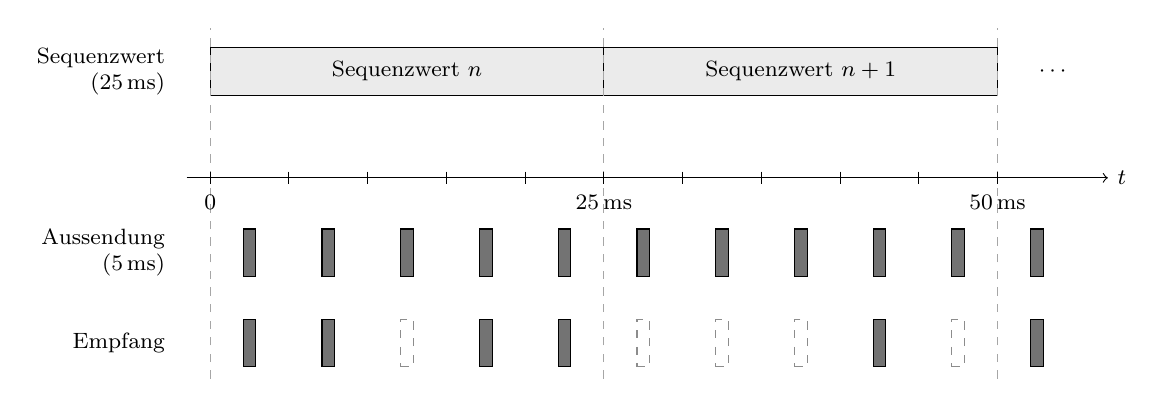
\begin{tikzpicture}[x=1cm, y=1cm,
        puls/.style  = {draw, fill=black!55, minimum width=0.16cm,
                        minimum height=0.6cm, inner sep=0pt},
        fehlt/.style = {draw=black!45, dashed, fill=none, minimum width=0.16cm,
                        minimum height=0.6cm, inner sep=0pt},
        rand/.style  = {draw=black!35, dashed},
        zeile/.style = {font=\footnotesize, align=right, anchor=east}]

        % Sequenzfenster
        \draw[fill=black!8] (0,1.05) rectangle (5,1.65);
        \draw[fill=black!8] (5,1.05) rectangle (10,1.65);
        \node[font=\footnotesize] at (2.5,1.35) {Sequenzwert $n$};
        \node[font=\footnotesize] at (7.5,1.35) {Sequenzwert $n+1$};
        \node[font=\footnotesize] at (10.7,1.35) {$\cdots$};

        % Trennlinien der Sequenzfenster
        \foreach \x in {0,5,10} \draw[rand] (\x,-2.55) -- (\x,1.9);

        % Zeitachse
        \draw[->] (-0.3,0) -- (11.4,0) node[right, font=\footnotesize] {$t$};
        \foreach \x in {0,1,2,3,4,5,6,7,8,9,10} \draw (\x,0.08) -- (\x,-0.08);
        \node[below, font=\footnotesize] at (0,-0.1)  {0};
        \node[below, font=\footnotesize] at (5,-0.1)  {25\,ms};
        \node[below, font=\footnotesize] at (10,-0.1) {50\,ms};

        % Sendetakt: alle 5 ms eine Aussendung
        \foreach \x in {0.5,1.5,2.5,3.5,4.5,5.5,6.5,7.5,8.5,9.5,10.5}
            \node[puls] at (\x,-0.95) {};

        % Empfang: einzelne Kopien fehlen
        \foreach \x in {0.5,1.5,3.5,4.5,8.5,10.5} \node[puls]  at (\x,-2.1) {};
        \foreach \x in {2.5,5.5,6.5,7.5,9.5}      \node[fehlt] at (\x,-2.1) {};

        % Zeilenbeschriftung
        \node[zeile] at (-0.45,1.35)  {Sequenzwert\\(25\,ms)};
        \node[zeile] at (-0.45,-0.95) {Aussendung\\(5\,ms)};
        \node[zeile] at (-0.45,-2.1)  {Empfang};
    \end{tikzpicture}
    \caption{Getrennte Taktung der Mess-Firmware. Je Sequenzwert werden fünf Kopien
        ausgesendet. Im dargestellten Verlauf gehen im ersten Fenster eine und im
        zweiten vier Kopien verloren, ohne dass ein Sequenzwert ausfällt. Als
        Sequenzverlust zählt erst ein Fenster, aus dem keine einzige Kopie eintrifft.}
    \label{fig:messtakte}
\end{figure}

Der Empfänger registriert einen ESP-NOW-Empfangs-Callback und wertet
jedes eingegangene Paket aus. Aus der Zählfolge wird zum einen
rekonstruiert, welche Sequenzwerte vollständig ausgeblieben sind, zum
anderen, wie viele der fünf Aussendungen je Sequenzwert tatsächlich
eingetroffen sind. Die erste Größe beschreibt den für die Lichtausgabe
maßgeblichen Verlust, die zweite die verbleibende Übertragungsreserve.
Zusätzlich werden die Länge der längsten zusammenhängenden Verlustserie,
die mittlere Zwischenankunftszeit aufeinanderfolgender Sequenzwerte und
deren Standardabweichung (Jitter) sowie die Empfangsfeldstärke (RSSI)
erhoben.
Der RSSI-Wert wird über einen im Promiscuous-Modus betriebenen
Paket-Sniffer ermittelt. Da Empfangs-Callback und Hauptschleife
gemeinsam auf die Zählvariablen zugreifen, wird dieser Zugriff über einen
Spinlock synchronisiert. Der Empfänger gibt im Sekundentakt eine
CSV-Zeile aus, die sowohl fenster- als auch laufzeitbezogene Kennzahlen
enthält.

\subsection{Datenerfassung und Auswertung}
\label{subsec:datenerfassung}

Die serielle Ausgabe des Empfängers wird host-seitig über das Skript
\texttt{capture.sh} aufgezeichnet, das den seriellen Port direkt ausliest
und die Aufzeichnung auf eine vorgegebene Dauer begrenzt, während die
Firmware selbst zeitlich unbegrenzt läuft. Die Rohdaten werden unverändert
als CSV abgelegt und nicht nachträglich modifiziert, um die
Reproduzierbarkeit der Auswertung zu gewährleisten.

Die Auswertung erfolgt über das Python-Skript \texttt{analyze.py}, das
jede Rohdatendatei verarbeitet und den Testtyp sowie die Messbedingungen
aus dem Dateinamen ableitet. Unterstützt werden die Testtypen
Paketverlust, Störfestigkeit, Reichweite und Langzeitstabilität, wobei
die Reichweitenmessung zusätzlich zwischen Läufen mit und ohne
Sichtverbindung unterscheidet und beide als getrennte Messreihen
auswertet. Das Skript erzeugt daraus Kennzahltabellen im \LaTeX- und
CSV-Format sowie Diagramme im PDF-Format, die direkt in die Arbeit
eingebunden werden. Berechnet werden die kumulierte und die
fensterbezogene Verlustrate, die mittlere Anzahl empfangener Kopien je
Sequenzwert, die längste Verlustserie, der Jitter sowie die mittlere
Feldstärke. Die Bedeutung dieser Kennzahlen für die Bewertung der
Lichtausgabe wird in Abschnitt~\ref{subsec:metriken} erläutert.

\section{Hardware-Design}
\label{sec:hardware-design}

Das Hardware-Design des Systems umfasst drei Leiterplatten:
das Bridge-PCB, das Tube-PCB sowie die Interface-PCB.
Letztere wird als gemeinsames, identisches Bedienelement sowohl
in der Bridge als auch in der Tube eingesetzt. Im Folgenden
werden zunächst die übergreifenden Fertigungs- und
Entwurfsparameter beschrieben, bevor die einzelnen Baugruppen
sowie die Leistungs-, Funk- und Schutzbeschaltung im Detail
erläutert werden.

\subsection{Leiterplattenfertigung und Entwurfsparameter}
\label{subsec:pcb-fertigung}

Der Schaltplan- und Leiterplattententwurf erfolgte mit dem
Open-Source-Software KiCad. Alle Platinen sind als
zweilagige Leiterplatten mit einer Kupferauflage von 35~µm
(1~oz/ft²) ausgeführt. Fertigung und Bestückung wurden über
den Dienstleister JLCPCB realisiert. Die Bestückung umfasst
eine Mischung aus SMD-Bauteilen der Baugröße 1206, die für
die manuelle Handlötung geeignet sind, sowie bedrahteten
THT-Komponenten an mechanisch belasteten Verbindungen wie
Steckverbindern.

Die Leiterbahnbreiten wurden last- und signalabhängig
ausgelegt. Leistungsleitungen der 12-V-Versorgung sind mit
2~mm Breite ausgeführt, um Ströme bis 4~A bei einer
zulässigen Temperaturerhöhung von 20~K sicher zu führen.
Dieser Wert ergibt sich gemäß IPC-2221 bei einer Kupferdicke
von 35~µm. Bei der umgesetzten Lösung mit 12V LED-Chips werden 
lediglich Ströme bis 2A erwartet. Um den Nachbau mit 5V Chips 
wie den weit verbreiteten WS2812b zu ermöglichen, bei welchen 
höhere Ströme bei gleicher Leistung fließen sind die 
Versorgungsleitungen entsprechend dimensioniert.
Signalleitungen sind mit 0,5~mm ausgeführt, da
dort deutlich geringere Ströme fließen. Alle übrigen
Designregeln orientieren sich an den Herstellervorgaben von
JLCPCB hinsichtlich minimaler Leiterbahnbreite und
minimalem Leiterabstand.

Ein besonderes Entwurfsmerkmal betrifft die Bridge: Deren DMX-Eingang
ist galvanisch vom übrigen Teil der Schaltung getrennt, was sich im
Layout in zwei voneinander abgesetzten Masseflächen niederschlägt. Die
konstruktive Umsetzung dieser Trennung wird in
Abschnitt~\ref{subsec:bridge-pcb} beschrieben.

Der Platinen-Formfaktor wurde an die jeweilige Gehäuse- und
Rohrgeometrie angepasst. Die Programmierung der ESP-Module 
sowie die serielle Diagnoseausgabe erfolgen
über den USB-C-Anschluss der jeweiligen Entwicklungsmodule.

\subsection{Bridge-PCB}
\label{subsec:bridge-pcb}

Die Bridge-Hauptplatine trägt den ESP32 DevKitC als
Mikrocontroller, ein USR-ES1-Ethernet-Modul auf Basis des
W5500-Chips mit SPI-Schnittstelle sowie zwei SN75176BP
RS-485-Transceiver für den DMX-Ein- und -Ausgang. Die
Spannungsversorgung der Bridge erfolgt über den
USB-C-Anschluss des DevKitC-Moduls mit 5~V. Da die Bridge
keine hohen Lastströme liefert, ist die USB-Stromversorgung
für den Betrieb aller angeschlossenen Komponenten ausreichend
dimensioniert. Die boardinternen Kondensatoren des DevKitC
stabilisieren die Versorgungsspannung, sodass kein
zusätzlicher Spannungsregler erforderlich ist.

Der DMX-Eingang ist galvanisch vom Rest der Schaltung
getrennt. Hierzu werden ein 6N137-Optokoppler sowie ein
ADUM1201-Digitalisolator eingesetzt. Die Spannungsversorgung
der galvanisch isolierten Seite erfolgt über einen
TEA1-0505-DC/DC-Wandler, der die Potentialtrennung über die
Transformatorstrecke aufrechterhält und bis zu 1500~V~DC
isoliert \cite{tea1_datasheet}. Ergänzt wird die Trennung im
Layout durch eine 5~mm breite Trennbahn ohne
Durchkontaktierungen zwischen den beiden Masseflächen. Diese
physikalische Barriere verhindert im Falle von Überspannungen
oder Fehlanschlüssen die Ausbreitung von Störungen zu den
empfindlichen Komponenten der nicht-isolierten Seite. Der
DC/DC-Wandler bildet die einzige Stelle, an der die Barriere
konstruktiv überbrückt wird. Abbildung~\ref{fig:bridge_pcb} zeigt die
Anordnung im Leiterplattenlayout.

\begin{figure}[H]
  \centering
  \includegraphics[width=0.75\linewidth]{images/bridge_pcb.png}
  \caption{Leiterplattenlayout der Bridge}
  \label{fig:bridge_pcb}
\end{figure}

Der DMX Ein- und Ausgang ist über
XLR-Einbaubuchsen (NC3MAH bzw. NC3FAH) zugänglich. Für eine mögliche
zukünftige Erweiterung um einen kabelgebundenen
Pixelsteuerungsmodus über Art-Net ist darüber hinaus ein
JST-XH-3-Pin-Ausgang für die WS2815-LED-Datenleitung
vorgesehen. Das Signal wird dabei durch einen
SN75176BP-Transceiver in ein RS-485-Differentialsignal
gewandelt, um eine störungsarme Übertragung über längere
Kabelstrecken zu ermöglichen. Diese Erweiterung ist nicht
Gegenstand der vorliegenden Arbeit.

Tabelle~\ref{tab:pinbelegung-bridge} fasst die Zuordnung der Signale zu
den GPIO-Pins zusammen. Da im Projekt ausschließlich der DMX-Empfang
benötigt wird, teilen sich Sendeleitung und Treiberfreigabe des
RS-485-Transceivers einen Pin, dadurch bleibt ein weiterer GPIO frei.

\begin{table}[H]
    \centering
    \small
    \begin{tabular}{lll}
        \toprule
        Baugruppe & Signal & GPIO \\
        \midrule
        DMX512 (RS-485)      & Empfang (RX)              & 16 \\
                             & Senden / Treiberfreigabe  & 17 \\
        Ethernet (W5500)     & Reset                     & 4  \\
                             & SPI Chip Select           & 5  \\
                             & SPI Takt                  & 18 \\
                             & SPI MISO                  & 19 \\
                             & SPI MOSI                  & 23 \\
        Interface-PCB        & I2C SCL                   & 25 \\
                             & I2C SDA                   & 26 \\
                             & Taster UP                 & 27 \\
                             & Taster DOWN               & 32 \\
                             & Taster ENTER              & 33 \\
        LED-Datenausgang     & Daten (vorbereitet)       & 14 \\
        \bottomrule
    \end{tabular}
    \caption{Pinbelegung der Bridge (ESP32 DevKitC).}
    \label{tab:pinbelegung-bridge}
\end{table}


\subsection{Tube-PCB}
\label{subsec:tube-mainboard}

Die Tube-Hauptplatine trägt den Seeed XIAO ESP32-S3 als
Mikrocontroller. Die Eingangsversorgung der Tube erfolgt mit
12~V, die über einen Step-Down-Buck-Converter auf 5~V für das
ESP32-Modul gewandelt werden. Das XIAO-Modul verfügt über
einen integrierten Pegelwandler, sodass die 5~V direkt am
VCC-Pin des Moduls angelegt werden können. Periphere
Komponenten wie das OLED-Display und die Taster werden intern
mit der geregelten 3,3~V-Spannung des ESP32 versorgt.

Zum Schutz vor Verpolung ist eine Schottky-Diode in der
12-V-Eingangsleitung verbaut. Eine zweite Schottky-Diode
zwischen dem Ausgang des Buck-Converters und dem VCC-Pin des
ESP32-Moduls verhindert eine Rückspeisung in den Converter,
wenn das Modul für Firmware-Updates über USB-C extern mit
Strom versorgt wird. Zur Stabilisierung der
Versorgungsspannungen sind Bulk-Kondensatoren im
Versorgungspfad vorgesehen.

Die 12-V-Leiterbahn zwischen Versorgungseingang und
LED-Strip-Ausgang folgt der in
Abschnitt~\ref{subsec:pcb-fertigung} beschriebenen Auslegung für
Leistungsleitungen, sie führt damit den in
Abschnitt~\ref{subsec:leistung-led} berechneten Betriebsstrom mit
deutlicher Reserve.

\begin{figure}[H]
  \centering
  \includegraphics[width=0.5\linewidth]{images/tube_power_supply_schematic.png}
  \caption{Versorgungspfad der Leuchtröhre}
  \label{fig:tube_power_supply}
\end{figure}

Die Verbindung zur Stromversorgung und zum LED-Strip erfolgt
über JST-VH-Steckverbinder, die laut Herstellerangaben eine
Belastbarkeit von bis zu 10~A bei 250~V AC/DC aufweisen und
damit für die vorliegenden Betriebsströme ausreichend
dimensioniert sind. Auf kleinere JST-XH Verbindungen wurde verzichtet,
um im Nachbau 5V Chips zu ermöglichen. \cite{jst_vh_datasheet}.

Tabelle~\ref{tab:pinbelegung-tube} zeigt die Pinbelegung der Röhre. Sie
fällt deutlich schlanker aus als bei der Bridge, da die Röhre keine
kabelgebundenen Steuerschnittstellen besitzt.

\begin{table}[H]
    \centering
    \small
    \begin{tabular}{lll}
        \toprule
        Baugruppe & Signal & GPIO \\
        \midrule
        LED-Strip     & Daten        & 4 \\
        Interface-PCB & I2C SCL      & 2 \\
                      & I2C SDA      & 3 \\
                      & Taster UP    & 7 \\
                      & Taster DOWN  & 9 \\
                      & Taster ENTER & 8 \\
        \bottomrule
    \end{tabular}
    \caption{Pinbelegung der Leuchtröhre (Seeed XIAO ESP32-S3).}
    \label{tab:pinbelegung-tube}
\end{table}

\subsection{Interface-PCB}
\label{subsec:interface-pcb}

Die Interface-Platine ist als geräteübergreifendes
Bedienelement konzipiert und wird in identischer Ausführung
sowohl in der Bridge als auch in der Tube eingesetzt. Sie
trägt ein 0,96\char`\"-OLED-Display auf Basis des
SSD1306-Controllers mit I2C-Schnittstelle sowie drei
Kurzhubtaster für die Menünavigation (UP, DOWN, ENTER). Die
elektrische Verbindung zur jeweiligen Hauptplatine erfolgt
über einen JST-XH-7-Pin-Steckverbinder, über den I2C-Signale,
GPIO-Leitungen der Taster sowie die Versorgungsspannung
übertragen werden.

Die Wiederverwendung einer identischen Bedienplatine in beiden
Gerätevarianten ist eine bewusste Designentscheidung: Sie
reduziert den Entwicklungs- und Fertigungsaufwand, da
lediglich eine Platine entwickelt, qualifiziert und gefertigt
werden muss, und stellt gleichzeitig eine konsistente
Bedienlogik auf beiden Gerätetypen sicher.

\subsection{Leistungsdimensionierung und LED-Auswahl}
\label{subsec:leistung-led}

Als LED-Typ wurde der WS2815 mit einer Betriebsspannung von
12~V gewählt. Gegenüber verbreiteten 5V-Typen wie dem WS2812
ergibt sich bei gleicher abgegebener Lichtleistung ein
geringerer Betriebsstrom, da die höhere Versorgungsspannung
eine entsprechend niedrigere Stromstärke erfordert. Der
ohmsche Spannungsabfall entlang des LED-Strips fällt dadurch
bei gegebener Leitungslänge kleiner aus, sodass auf eine
beidseitige Einspeisung der Versorgungsspannung
verzichtet werden kann. Dies vereinfacht die
Dimensionierung von Leiterbahnen, Zuleitungen und Netzteil.
Da die WS2815-IC-Chips das gleiche Protokoll wie die WS2812 verwenden, ist die
Ansteuerung mit der \texttt{FastLED}-Bibliothek ohne Anpassungen
möglich \cite{ws2815_datasheet}. 
Zudem haben sie als Weiterentwicklung einen redundanten Datenkanal,
der die LED-Kette auch bei einem Ausfall einzelner Pixel funktionsfähig
hält. Der Datenanschluss erwartet einen 5V-Logikpegel, während der
ESP32 mit 3,3~V ausgibt. Da der Schaltschwellwert des Eingangs knapp
unterhalb dieses Werts liegt, arbeitet die direkte Ansteuerung im
aufgebauten System zuverlässig, sodass auf einen Pegelwandler verzichtet
wurde.
Jeder WS2815-Schaltkreis steuert ein einzelnes LED-Pixel und
bestimmt damit die räumliche Auflösung entlang des Rohrs.

Das Strombudget ergibt sich aus der Anzahl der Pixel
multipliziert mit der maximalen Leistung pro Pixel. Bei voller
Helligkeit (Weiß, alle drei Farbkanäle voll ausgesteuert)
nimmt ein Pixel maximal 0,2~W auf. Für einen
LED-Strip mit 120~Pixeln ergibt sich damit eine
Gesamtleistungsaufnahme von 24~W, entsprechend einem Strom
von 2~A bei 12~V (vgl. Abschnitt~\ref{subsec:elektrische-belastbarkeit}).
Die 12-V-Versorgungsleitung ist mit 2~mm Breite auf 4~A ausgelegt
(Abschnitt~\ref{subsec:pcb-fertigung}) und führt den Betriebsstrom damit
mit dem Faktor zwei an Reserve.

Die LEDs werden direkt aus der 12-V-Versorgung gespeist. Der
Buck-Converter versorgt ausschließlich die Logikkomponenten
(ESP32, OLED-Display, Taster).

\subsection{Funkanbindung und Antennenführung}
\label{subsec:funk-antenne}

Die Funkübertragung der ESP-Module erfolgt über extern
angeschlossene Antennen, die über SMA-Steckverbinder mit den
Modulen verbunden sind. Bei der Bridge wird die Antenne aus
dem Gehäuse herausgeführt, um Abschirmungseffekte durch das
Gehäusematerial zu minimieren und eine maximale
Abstrahlleistung zu den Röhren zu erzielen. Als
Senderantenne wird eine Stabantenne mit einem vom Hersteller
angegebenen Gewinn von etwa 9~dBi eingesetzt. Dieser Wert ist
herstellerseitig nicht durch ein Messprotokoll belegt und daher als
Richtgröße zu verstehen. Die Antenne ist auf das
2,4-GHz-Band ausgelegt und
gegenüber den integrierten Chiplantennen der ESP-Module eine
deutlich verbesserte Richtcharakteristik und somit größere
Reichweite bietet.

An den Röhren wird aufgrund der räumlichen Einschränkungen
durch das Rohrgehäuse eine kompakte flexible Antenne mit
15~cm Länge verwendet. Bei der Montage ist darauf zu achten,
dass die Antenne möglichst gerade im Gehäuse verläuft und
nicht von abschirmenden Materialien umgeben ist. Die Antenne
ist am Rohrende platziert, sodass die Abstrahlung durch das
nichtmetallische Polycarbonat erfolgt, welches hochfrequente
Signale im 2,4-GHz-Bereich ohne nennenswerte Dämpfung
passiert. Die rückseitige Abstrahlung wird durch das
Aluminiumprofil des Rohrs begrenzt, was für den typischen
Veranstaltungsbetrieb, bei dem die Bridge frontal zu den
Röhren positioniert wird, unkritisch ist. Der Einfluss der
Antennenanordnung auf Reichweite und Empfangsfeldstärke wird
in Kapitel~\ref{chap:evaluierung} quantitativ bewertet.

\subsection{Schutzbeschaltung und Signalintegrität}
\label{subsec:schutz-signalintegritaet}

Auf der Bridge ist die RS-485-Busleitung des DMX-Eingangs
mit einem 120-Ω-Abschlusswiderstand terminiert, um
Leitungsreflexionen bei langen Kabelstrecken zu vermeiden.
Den Schutz der nach außen geführten XLR-Anschlüsse übernimmt
primär die galvanische Trennung des DMX-Eingangs
(vgl. Abschnitt~\ref{subsec:bridge-pcb}): Optokoppler und
Digitalisolator unterbrechen den leitenden Pfad zur übrigen
Schaltung, sodass sowohl leitungsgebundene Störungen als auch
elektrostatische Entladungen die empfindlichen Komponenten
nicht erreichen. Zusammen mit der 5-mm-Trennbahn im Layout
ergibt sich daraus eine zweistufige Schutzstrategie.

Der Verpolschutz der Tube-Platine wird über eine
Schottky-Diode in der Eingangsleitung realisiert
(vgl. Abschnitt~\ref{subsec:tube-mainboard}).

Die LED-Datenleitung ist unmittelbar am Signalausgang des
Mikrocontrollers mit einem 330-Ω-Serienwiderstand beschaltet,
um Signalflanken zu dämpfen und hochfrequente Reflexionen auf
der Leitung zu reduzieren. 
Kondensatoren mit 100\,µF und 100\,nF sind sowohl am Spannungseingang
der Tube-Platine als auch am LED-Strip-Ausgang vorgesehen,
um die Versorgungsspannung zu stabilisieren und hochfrequente
Störungen zu unterdrücken.

\subsection{Thermisches Design}
\label{subsec:thermik}

Die LEDs stellen die dominante Wärmequelle im System dar. Im
Inneren des geschlossenen Polycarbonatrohrs ist die natürliche
Konvektion stark eingeschränkt, sodass die entstehende Wärme
vorrangig über das Aluminiumprofil, auf dem der LED-Strip
aufgebracht ist, an die Umgebung abgeleitet wird. Das
Aluminiumprofil übernimmt damit neben seiner Funktion als
mechanischer Träger gleichzeitig die Rolle eines passiven
Kühlkörpers.

Der im Tube-Mainboard verbaute Buck-Converter trägt ebenfalls
zur Wärmeentwicklung bei. Da er im vorliegenden System
ausschließlich die Logikkomponenten versorgt, ist seine
Verlustleistung im Vergleich zur LED-Last gering. Die
Platzierung des Converters auf der Platine berücksichtigt
einen ausreichenden Abstand zu wärmeempfindlichen Bauteilen.

\section{Mechanischer Aufbau und Gehäuse}
\label{sec:gehaeuse}


Die Gehäuse für die Bridge und die Tube-Enden sind als
3D-gedruckte Bauteile ausgeführt. Die zugehörigen Druckdateien
im 3MF-Format sind im Projektrepository hinterlegt. Da
3D-gedruckte Bauteile aus schichtweise abgelegtem Kunststoff
orthotrope Festigkeitseigenschaften aufweisen, die
Festigkeit in Schichtrichtung ist also geringer als quer dazu,
wird das Tube-Gehäuse liegend gedruckt, sodass die
Schichtgrenzen parallel zur dominanten Biegebelastung
orientiert sind. Das maßgebliche Biegemoment entsteht durch
horizontale Kräfte, wenn die Röhre über den Gewindeeinsatz
ihres Standfußes gehalten wird. Eine zur Belastungsrichtung
ungünstig orientierte Schichtstruktur würde hingegen zur
Delamination entlang der Schichtgrenzen führen.

Die Leiterplatten werden über wärmeeingebettete
Schraubgewindeeinsätze (M2 für die Interface-PCB, M3 für
Bridge- und Tube-Mainboard) im Gehäuse befestigt. Dieses
Verfahren verbindet den Metallgewindeeinsatz stoffschlüssig
mit dem Kunststoff und bietet eine deutlich höhere
Ausreißfestigkeit als direkt in den Kunststoff geschnittene
Gewinde.

\begin{figure}[H]
  \centering
  \includegraphics[width=0.25\linewidth]{images/tube_querschnitt.png}
  \caption{Querschnitt der Leuchtröhre}
  \label{fig:tube_querschnitt}
\end{figure}

Der LED-Strip ist auf einem Aluminiumprofil montiert, das als
mechanischer Träger im Inneren des Polycarbonatrohrs verläuft
und gleichzeitig als passive Wärmesenke dient
(vgl. Abschnitt~\ref{subsec:thermik}). Das Polycarbonatrohr
ist in einer opalen Ausführung gewählt, um
das emittierte Licht zu streuen und ein gleichmäßiges
Leuchtbild ohne sichtbare Einzelpixel zu erzeugen. Die Kabel
an den Rohrenden sind durch Klebstoff zugentlastet, der das
Kabel am Ausführungspunkt fixiert und mechanische Zug- und
Biegebelastungen von den Lötstellen auf der Platine fernhält.

Für den Bühneneinsatz ermöglicht das Aluminiumprofil neben der
LED-Befestigung auch das Rigging der Röhre: Über eine in das
Profil integrierte Nut kann die Röhre hängend oder stehend
montiert werden.

\section{Stücklisten und Kostenabschätzung}
\label{sec:stuecklisten}
Kosten können variieren, abhängig von Bezugsquelle und Bestellmenge. 
Die angegebenen Preise beziehen sich auf Bestellungen für 20 Einheiten 
und dienen als grobe Orientierung für die Materialkosten pro Stück. 
Alle Preise verstehen sich inklusive Mehrwertsteuer und Versandkosten, 
basierend auf den Angeboten der Lieferanten zum Zeitpunkt der Erstellung dieser Arbeit.

\subsection{Stücklisten}
\label{subsec:stuecklisten-tabellen}

\begin{table}[H]
    \centering
    \begin{tabular}{|c|l|r|}
        \hline
        \textbf{Menge} & \textbf{Bauteil} & \textbf{Stückpreis} \\ \hline
        1x & Interface Platine (PCB) & 1.40 € \\ \hline
        1x & 0.96" OLED-Display (SSD1306) & 1.78 € \\ \hline
        3x & Kurzhubtaster 6x6mm & 0.06 € \\ \hline
        2x & M2 Schraubgewindeeinsatz & 0.10 € \\ \hline
        2x & M2 Schrauben & 0.10 € \\ \hline
        \multicolumn{2}{|r|}{\textbf{Summe:}} & \textbf{3.76 €} \\ \hline
    \end{tabular}
    \caption{Bauteilliste: Interface}
    \label{tab:bauteile_interface}
\end{table}

\begin{table}[H]
    \centering
    \begin{tabular}{|c|l|r|}
        \hline
        \textbf{Menge} & \textbf{Bauteil} & \textbf{Stückpreis} \\ \hline
        1x & Bridge Platine (PCB) & 1.60 € \\ \hline
        1x & Interface PCB + Bauteile & 3.76 € \\ \hline
        1x & ESP32 DevKitC & 8.25 € \\ \hline
        1x & USR-ES1 Ethernet-Modul (W5500) & 4.60 € \\ \hline
        2x & SN75176BP & 0.07 € \\ \hline
        1x & 6N137 & 0.30 € \\ \hline
        1x & ADUM 1201 & 0.30 € \\ \hline
        2x & TEA1-0505 & 0.49 € \\ \hline
        2x & 330 Ohm Widerstände (1206 SMD) & 0.02 € \\ \hline
        1x & NC3MAH & 2.15 € \\ \hline
        1x & NC3FAH & 1.88 € \\ \hline
        1x & JST-XH 3Pin Männlich / Gerade & 0.02 € \\ \hline
        1x & JST-XH 7Pin Männlich / Gerade & 0.22 € \\ \hline
        2x & M3 Schraubgewindeeinsatz & 0.10 € \\ \hline
        2x & M3 Schrauben & 0.10 € \\ \hline
        1x & SMA-Antenne & 6,35 € \\ \hline
        \multicolumn{2}{|r|}{\textbf{Summe:}} & \textbf{30.99 €} \\ \hline
    \end{tabular}
    \caption{Bauteilliste: Bridge}
    \label{tab:bauteile_bridge}
\end{table}

\begin{table}[H]
    \centering
    \begin{tabular}{|c|l|r|}
        \hline
        \textbf{Menge} & \textbf{Bauteil} & \textbf{Stückpreis} \\ \hline
        1x & Tube Platine (PCB) & 1.40 € \\ \hline
        1x & Interface PCB + Bauteile & 3.76 € \\ \hline
        1x & Xiao ESP32-S3 & 8.75 € \\ \hline
        1x & Step-Down Buck-Converter & 0.30 € \\ \hline
        1x & JST-VH 2Pin Männlich / Gewinkelt & 0.12 € \\ \hline
        1x & JST-VH 3Pin Männlich / Gewinkelt & 0.12 € \\ \hline
        1x & JST-XH 7Pin Männlich / Gerade & 0.22 € \\ \hline
        2x & Schottky-Diode 100V 2A SMA & 0.02 € \\ \hline
        1x & 470 $\mu$F Kondensator (1206 SMD) & 0.02 € \\ \hline
        1x & 100 $\mu$F Kondensator (1206 SMD) & 0.02 € \\ \hline
        3x & 100 nF Kondensator (1206 SMD) & 0.02 € \\ \hline
        1x & 330 Ohm Widerstand (1206 SMD) & 0.02 € \\ \hline
        2x & M3 Schraubgewindeeinsatz & 0.10 € \\ \hline
        2x & M3 Schrauben & 0.10 € \\ \hline
        1x & SMA-Antenne & 0.87 € \\ \hline
        1x & Polycarbonat Difusor 2m & 19.99 € \\ \hline
        1x & Aluminium Profil 2m & 9.99 € \\ \hline
        1x & 2m WS2815 LED-Strip (12V, 120 LEDs/m) & 10.88 € \\ \hline
        1x & 12V 5A Netzteil & 3.99 € \\ \hline
        1x & Gehäuse (3D-Druck) & 1.00 € \\ \hline
        \multicolumn{2}{|r|}{\textbf{Summe:}} & \textbf{62.09 €} \\ \hline
    \end{tabular}
    \caption{Bauteilliste: Tube}
    \label{tab:bauteile_tube}
\end{table}

\subsection{Gesamtkosten}
\label{subsec:gesamtkosten}

Die Gesamtkosten eines vollständigen Systems ergeben sich aus
der Summierung der Einzelbaugruppen einer Bridge sowie der
gewünschten Anzahl von Tubes. Auf Basis der in
Abschnitt~\ref{subsec:stuecklisten-tabellen} aufgeführten
Stücklisten betragen die Materialkosten pro Bridge ca. 31~€.
Die Tube kostet mit ca. 62~€ mehr als doppelt so viel.
Vor allem LED-Strip, Netzteil und Gehäuse treiben die Kosten in die Höhe.
Sollen die Kosten pro Tube gesenkt werden, steckt das Potenzial 
vor allem beim Diffusor und dem Aluprofil. Hier kann auf kostengünstigere 
Alternativen zurückgegriffen werden.